\chapter{Signal Processing in GPUs}
\label{chap:gpu}
A graphics processing unit (GPU) is a computational unit with a highly-parallel architecture well-suited for executing the same function on many data elements.
In the past, GPUs were used to process graphics data but in 2008 NVIDIA released the Tesla GPU.
Telsa GPUs are built for general purpose high performance computing.
Figure \ref{fig:GPUpicture} shows the form factor of a Tesla K40c and K20c.
\begin{figure}
	\centering\includegraphics[width=5in]{figures/gpu_intro/k40c_k20c.jpg}
	\caption{NVIDIA Tesla K40c and K20c.}
	\label{fig:GPUpicture}
\end{figure}

In 2007 NVIDIA released an extension to C, C++ and Fortran called CUDA (Compute Unified Device Architecture).
CUDA enables GPUs to be used for high performance computing in computer vision, deep learning, artificial intelligence, and signal processing \cite{wikipedia-gpu:2015}.
CUDA allows a programmer to write C++ like functions that are massively parallel called kernels.
To invoke parallelism, a GPU kernel executed $N$ times with the work distributed to $N_\text{min}$ total threads that run concurrently.
To achieve the full potential of high performance GPUs, kernels must be written with some basic concepts about GPU architecture and memory in mind.
This chapter will show the following:
\begin{itemize}
\item Optimizing memory access leads to faster execution time, rather than optimizing number of floating point operations.
\item The number of threads per block can significantly affect execution time.
\item CPU and GPU processing can be pipelined.
\item Convolution maps very well to GPUs using the Fast Fourier Transform (FFT).
\item Batched processing leads to faster execution time per batch.
\end{itemize}

\section{GPU and CUDA Introduction}
\subsection{An Example Comparing CPU and GPU}
If a programmer has some C++ experience, learning how to program GPUs using CUDA comes fairly easily.
GPU code still runs top to bottom and memory still has to be allocated.
The only real difference is the physical location of the memory and how functions run on GPUs.
To run functions or kernels on GPUs, the memory must be copied from the host (CPU) to the device (GPU).
Once the memory has been copied, parallel GPU kernels operate on the data.
After GPU kernel execution, results are usually copied back from the device (GPU) to the host (CPU).

Listing \ref{code:GPUvsCPU} shows a simple program that implements real-valued float vector addition in a CPU and a GPU.
The vector $\mathbf{C}_1$ is the sum of the vectors $\mathbf{A}_1$ and $\mathbf{B}_1$ computed in the CPU.
The vector $\mathbf{C}_2$ is the sum of the vectors $\mathbf{A}_2$ and $\mathbf{B}_2$ computed in the GPU.
Line $42$ the CPU computes $\mathbf{C}_1$ by summing elements of $\mathbf{A}_1$ and $\mathbf{B}_1$ together sequentially. Figure \ref{fig:CPUaddBlockDiagram} shows how the CPU 
sequentially computes one element of $\mathbf{C}_1$ at time by summing one element from $\mathbf{A}_1$ and one element $\mathbf{B}_1$.

The GPU performs all the summations in parallel because each element of $\mathbf{C}_2$ is independent of all other elements. 
Before the computation of $\mathbf{C}_2$ can execute on the GPU, the vectors in host memory $\mathbf{A}_1$ and $\mathbf{B}_1$ are copied to device memory vectors $\mathbf{A}_2$ and $\mathbf{B}_2$ as shown on lines $60$ and $61$.
Once $\mathbf{A}_2$ and $\mathbf{B}_2$ are on the GPU, the vector $\mathbf{C}_2$ is computed by calling the GPU kernel VecAddGPU on line $75$.
VecAddGPU computes all the elements of $\mathbf{C}_2$ by performing a summation of all the elements of $\mathbf{A}_2$ and $\mathbf{B}_2$.
The vector $\mathbf{C}_2$ is then copied from device memory to host memory on line $78$.
Figure \ref{fig:GPUaddBlockDiagram} shows how the GPU computes $\mathbf{C}_2$ in parallel.

\begin{figure}
	\centering\includegraphics[width=3.17in/100*55]{figures/gpu_intro/CPUaddBlockDiagram.pdf}
	\caption{A block diagram of how a CPU sequentially performs vector addition.}
	\label{fig:CPUaddBlockDiagram}
\end{figure}
\begin{figure}
	\centering\includegraphics[width=4.69in/100*55]{figures/gpu_intro/GPUaddBlockDiagram.pdf}
	\caption{A block diagram of how a GPU performs vector addition in parallel.}
	\label{fig:GPUaddBlockDiagram}
\end{figure}

\singlespacing
\clearpage
\begin{lstlisting}[style=myCUDAstyle,caption={Comparison of CPU and GPU code.},label={code:GPUvsCPU}]
#include <iostream>
#include <stdlib.h>
#include <math.h>
using namespace std;

void VecAddCPU(float* destination,float* source0,float* source1,int myLength){
	for(int i = 0; i < myLength; i++)
		destination[i] = source0[i] + source1[i];
}

__global__ void VecAddGPU(float* destination, float* source0, float* source1, int lastThread){
	int i = blockIdx.x*blockDim.x + threadIdx.x;

	// don't access elements out of bounds
	if(i >= lastThread)
		return;

	destination[i] = source0[i] + source1[i];
}

int main(){
	int N = pow(2,22);
	cout << N << endl;
	/**
	* Vector Addition on CPU
	*/
	// allocate memory on host
	float *A1;
	float *B1;
	float *C1;
	A1 = (float*) malloc (N*sizeof(float));
	B1 = (float*) malloc (N*sizeof(float));
	C1 = (float*) malloc (N*sizeof(float));

	// Initialize vectors 0-99
	for(int i = 0; i < N; i++){
		A1[i] = rand()%100;
		B1[i] = rand()%100;
	}

	// vector sum C1 = A1 + B1
	VecAddCPU(C1, A1, B1, N);
	
	/**
	* Vector Addition on GPU
	*/
	// allocate memory on host for result
	float *C2;
	C2 = (float*) malloc (N*sizeof(float));

	// allocate memory on device for computation
	float *A2_gpu;
	float *B2_gpu;
	float *C2_gpu;
	cudaMalloc(&A2_gpu, sizeof(float)*N);
	cudaMalloc(&B2_gpu, sizeof(float)*N);
	cudaMalloc(&C2_gpu, sizeof(float)*N);

	// Copy vectors A and B from host to device
	cudaMemcpy(A2_gpu, A1, sizeof(float)*N, cudaMemcpyHostToDevice);
	cudaMemcpy(B2_gpu, B1, sizeof(float)*N, cudaMemcpyHostToDevice);

	// Set optimal number of threads per block
	int T_B = 32;

	// Compute number of blocks for set number of threads
	int B = N/T_B;

	// If there are left over points, run an extra block
	if(N % T_B > 0)
		B++;

	// Run computation on device
	//for(int i = 0; i < 100; i++)
	VecAddGPU<<<B, T_B>>>(C2_gpu, A2_gpu, B2_gpu, N);

	// Copy vector C2 from device to host
	cudaMemcpy(C2, C2_gpu, sizeof(float)*N, cudaMemcpyDeviceToHost);

	// Compare C2 to C1
	bool equal = true;
	for(int i = 0; i < N; i++)
		if(C1[i] != C2[i])
			equal = false;
	if(equal)
		cout << "C2 is equal to C1." << endl;
	else
		cout << "C2 is NOT equal to C1." << endl;

	// Free vectors on CPU
	free(A1);
	free(B1);
	free(C1);
	free(C2);

	// Free vectors on GPU
	cudaFree(A2_gpu);
	cudaFree(B2_gpu);
	cudaFree(C2_gpu);
}
\end{lstlisting}
\doublespacing

\subsection{GPU Kernel Using Threads and Thread Blocks}
A GPU kernel is executed by launching blocks with a set number of threads per block.
In the Listing \ref{code:GPUvsCPU}, VecAddGPU is launched on line 75 with $32$ threads per block.
The total number of threads launched on the GPU is the number of blocks times the number of threads per block.
VecAddGPU needs to be launched with at least $N = 2^{22}$ (line 22) threads or $2^{22}/32$ blocks of $32$ threads.

CUDA gives each thread launched in a GPU kernel a set of unique indices called threadIdx and blockIdx.
threadIdx is the thread index inside the assigned thread block.
blockIdx is the index of the block to which the thread is assigned.
Both threadIdx and blockIdx are three dimensional (i.e., they both have $x$, $y$, and $z$ components).
In this thesis only the $x$ dimension is used, because the GPU kernels operate only on one dimensional vectors.
blockDim is the number of threads assigned per block, in fact blockDim is equal to the number of threads per block because the vectors are one dimensional.

To convert the CPU ``for loop'' on line 7 to a GPU kernel, at least $N$ threads are launched with $T$ threads per thread block.
The number of blocks needed is $B = \frac{N}{T_B}$ or $B = \frac{N}{T}+1$, if $N$ is not an integer multiple of $T$.
Figure \ref{fig:threadsBlocks32} shows $N = 32$ threads launched in $B = 4$ thread blocks with $T = 8$ threads per block.
Figure \ref{fig:threadsBlocks36} shows $N = 36$ threads launched in $B = 5$ thread blocks with $T = 8$ threads per block. 
An full extra thread block is launched with $T = 8$ threads, but $4$ threads are idle.
Thread blocks are executed independent of other thread blocks.
The GPU does not guarantee Block $0$ will execute before Block $2$.
\begin{figure}
	\centering\includegraphics[width=4in/100*55]{figures/gpu_intro/threadsBlocks32.pdf}
	\caption{$32$ threads launched in $4$ thread blocks with $8$ threads per block.}
	\label{fig:threadsBlocks32}
\end{figure}
\begin{figure}
	\centering\includegraphics[width=5in/100*55]{figures/gpu_intro/threadsBlocks36.pdf}
	\caption{$36$ threads launched in $5$ thread blocks with $8$ threads per block with $4$ idle threads.}
	\label{fig:threadsBlocks36}
\end{figure}

\subsection{GPU Memory}
\label{sec:GPU_memory}
GPUs have plenty of computational resources, but most GPU kernels are limited by memory bandwidth to feed the computational units.
GPU kernels execute faster if the kernel is designed to access memory efficiently, rather than reducing the computational burden.
NVIDIA GPUs have many different types of memory to maximize speed and efficiency.

The fastest memory is private local memory,
in the form of Registers and L1 Cache/shared memory.
Local memory is fast, but only kilobytes are available.
The slowest memory is public memory in the form of the L2 Cache and Global Memory.
Public memory is slow, but gigabytes are available.
Figure \ref{fig:MemoryPyramid} shows the trade-off of memory speed and the size of different types of memory.
\begin{figure}
	\centering\includegraphics[width=8.36in/100*55]{figures/gpu_intro/MemoryPyramid.pdf}
	\caption{Diagram comparing memory size and speed. Global memory is massive but extremely slow. Registers are extremely fast but there are very few.}
	\label{fig:MemoryPyramid}
\end{figure}

Figure \ref{fig:GPUarch} shows a picture of the GPU hardware.
The solid boxes show that the L2 cache and Global Memory are physically located off the GPU chip. 
The dashed box shows that Registers and L1 Cache/Shared Memory are physically located \textit{on} the GPU chip. 
A public memory access takes over 60 clock cycles, because the memory is off chip. 
A local memory access is only a few clock cycles because the memory is on chip.
\begin{figure}
	\centering\includegraphics[width=\textwidth]{figures/gpu_intro/Kepler_box.png}
	\caption{Example of an NVIDIA GPU card. The GPU chip with registers and L1/shared memory is shown in the dashed box.	The L2 cache and global memory is shown off chip in the solid boxes.}
	\label{fig:GPUarch}
\end{figure}

Figure \ref{fig:fullGPUmemBlockDiagram} illustrates where each type of memory is located.
Threads have access to their own Registers and the L1 Cache.
Threads in a block can coordinate using shared memory, because shared memory is private to the thread block.
All threads have access to the L2 Cache and Global Memory.
The figure also shows that thread blocks are assigned to streaming multiprocessors (SMs).
CUDA handles all the thread block assignments to SMs.
\begin{figure}
	\centering\includegraphics[width=9.83in/100*55]{figures/gpu_intro/fullGPUmemBlockDiagram.pdf}
	\caption{A block diagram where local, shared, and global memory is located. Each thread has private local memory. Each thread block has private shared memory. The GPU has global memory that all threads can access.}
	\label{fig:fullGPUmemBlockDiagram}
\end{figure}
Table \ref{tab:gpu-resources_jeffs} lists Telsa K40c and K20c resources.
\begin{table}
\caption{The resources available with three NVIDIA GPUs used in this thesis (1x Tesla K40c 2x Tesla K20c). Note that CUDA configures the size of the L1 cache needed.}
\begin{center}
\begin{tabular}{llll}
	\toprule
	Feature 			& Per			& Tesla K40c 	& Tesla K20c	\\ \midrule
	Global Memory 		& GPU			& 12 GB	 		& 5 GB			\\
	L2 Cache Size 		& GPU			& 1.6 GB		& 1.3 GB		\\
	Memory Bandwidth	& 				& 288 GB/s		& 208 GB/s		\\		
	Shared Memory 		& Thread Block	& 49 kB			& 49 kB			\\
	L1 Cache Size 		& Thread Block	& variable		& variable		\\
	Registers			& Thread Block	& 65536			& 65536			\\
	Maximum Threads		& Thread Block	& 1024			& 1024			\\
	CUDA Cores 			& GPU			& 2880 			& 2496 			\\
	Base Core Clock 	&				& 745 MHz 		& 732 MHz		\\ \bottomrule
\end{tabular}
\end{center}
\label{tab:gpu-resources_jeffs}
\end{table}

\subsection{Thread Optimization}
Most resources listed in Table \ref{tab:gpu-resources_jeffs} show how much memory per thread block is available. 
The number of threads per block and the amount of resources available have an inverse relationship.
Threads have very little memory resources available, if a GPU kernel launches 1024 threads per block.
Threads have a lot of memory resources available, if a GPU kernel launches 32 threads per block.
This section shows that finding the optimum number of threads per block can dramatically speed up GPU kernels.

Improving memory accesses should always be the first optimization, when a GPU kernel needs to be faster.
The next step is to find the optimal number of threads per block to launch.
Knowing the perfect number of threads per block to launch is challenging to calculate.
Fortunately, the maximum number of possible threads per block is $1024$ in the Tesla K40c and K20c GPUs.
Listing \ref{code:threadTiming} shows a simple test program that measures GPU kernel execution time, while varying the number of possible threads per block.
The number of threads per block with the fastest computation time is the optimal number of threads per block for that specific GPU kernel.

\singlespacing
\begin{lstlisting}[style=myCUDAstyle,caption={Code snippet for thread optimization.},label={code:threadTiming}]
float milliseconds_opt = pow(2,10); // initiaize to "big" number
int T_B_opt;
int minNumTotalThreads = pow(2,20); // set to minimum number of required threads
for(int T_B = 1; T_B<=1024; T_B++){
	int B = minNumTotalThreads/T_B;
	if(minNumTotalThreads % T_B > 0)
		B++;
	cudaEvent_t start, stop;
	cudaEventCreate(&start);
	cudaEventCreate(&stop);
	cudaEventRecord(start);
	
	GPUkernel<<<B, T_B>>>(dev_vec0, dev_vec1);
	
	cudaEventRecord(stop);
	cudaEventSynchronize(stop);
	float milliseconds = 0;
	cudaEventElapsedTime(&milliseconds, start, stop);
	cudaEventDestroy(start);
	cudaEventDestroy(stop);
	if(milliseconds<milliseconds_opt){
		milliseconds_opt = milliseconds;
		T_B_opt = T_B;
	}
}
cout << "Optimal Threads Per Block " << T_B_opt << endl
cout << "Optimal Execution Time    " << milliseconds_opt << endl;
\end{lstlisting}
\doublespacing

Most of the time the optimal number of threads per block is a multiple of $32$ this is because
at the lowest level of architecture, GPUs perform computations in warps.
Warps are groups of $32$ threads that perform every computation together in lock step.
If the number of threads per block is not a multiple of $32$, some threads in a warp are idle and the GPU has unused computational resources.

Figure \ref{fig:ConvGPU_shared_12672_186taps} shows the execution time of an example GPU kernel.
The optimal execution time is $0.1078$ ms at the optimal $96$ threads per block.
By simply adjusting the number of threads per block, the execution time of this example kernel can be reduced by a factor of 2.

Adjusting the number of threads per block does not always dramatically reduce execution time.
Figure \ref{fig:ConvGPU_global_12672_186taps} shows the execution time for another GPU kernel with varying threads per block.
The execution time of this example kernel can be reduced by 1.12 by launching $560$ threads per block.
\begin{figure}
	\centering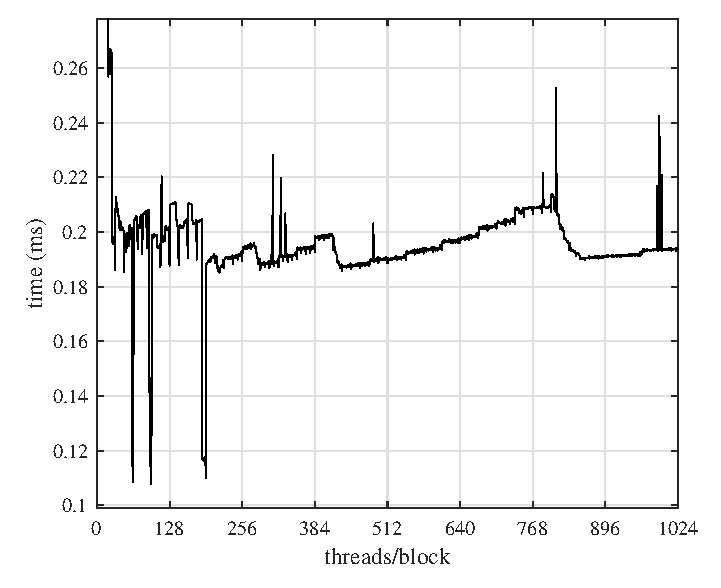
\includegraphics[width=5in]{figures/gpu_intro/ConvGPU_shared_12672_186taps.eps}
	\caption{Plot showing how execution time is affected by changing the number of threads per block.
	The optimal execution time for an example GPU kernel is $0.1078$ ms at the optimal $96$ threads per block.}
	\label{fig:ConvGPU_shared_12672_186taps}
\end{figure}
\begin{figure}
	\centering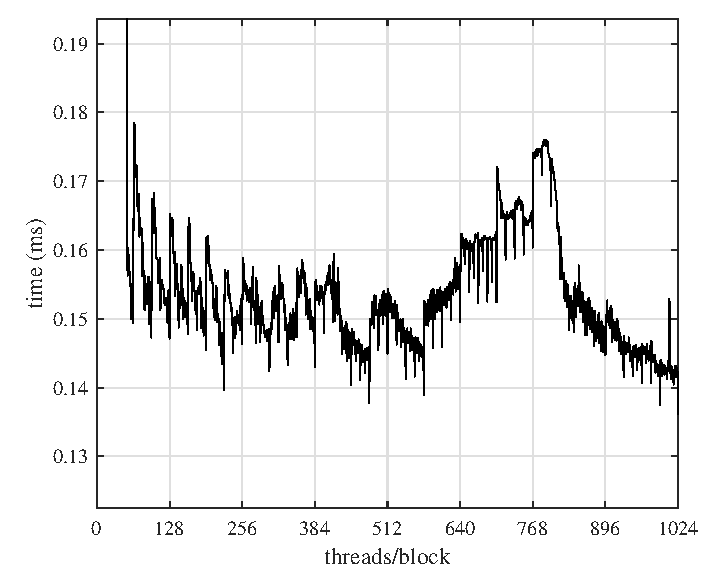
\includegraphics[width=5in]{figures/gpu_intro/ConvGPU_global_12672_186taps.eps}
	\caption{Plot showing the number of threads per block doesn't always drastically affect execution time.}
	\label{fig:ConvGPU_global_12672_186taps}
\end{figure}

While designing a custom GPU kernel to obtain a major speed up is satisfying,
CUDA has optimized GPU libraries that are extremely useful and efficient with exceptional documentation.
The CUDA libraries are written by NVIDIA engineers to maximize the performance of NVIDIA GPUs.
The libraries explained in this thesis include cuFFT, cuBLAS and cuSolverSp.

\subsection{CPU and GPU Pipelining}
While GPU kernels execute physically on the GPU, the GPU only executes instructions received from the host CPU.
The CPU is idle while it waits for GPU kernels to execute.
To introduce CPU and GPU pipelining, the CPU can be pipelined by performing other operations while waiting for the GPU to finish executing kernels.

A basic CPU GPU program with no pipelining is shown in Listing \ref{code:noPipe}.
The CPU acquires data from myADC on Line 5.
After the CPU takes time to acquire data, the data is copied from the host (CPU) to the device (GPU) on line 8.
The data is processed on the GPU once then the result is copied back to the device to host on line 9 and 10.
The cudaDeviceSynchronize function on line 13 blocks CPU until all GPU instructions are finished executing.
Note that the CPU is blocked during any host to device or device to host transfer.
Acquiring and copying data takes processing time on the CPU and GPU.
Figure \ref{fig:concurrentCPU_blocking} shows a block diagram of what is happening on the CPU and GPU in Listing \ref{code:noPipe} (end of the section).
The GPU is idle while the CPU is acquiring data and the CPU is idle while the GPU is processing.
\begin{figure}
	\centering\includegraphics[width=8.77in/100*55]{figures/gpu_intro/concurrentCPU_blocking.pdf}
	\caption{The typical approach of CPU and GPU operations. This block diagram shows the profile of Listing \ref{code:noPipe}.}
	\label{fig:concurrentCPU_blocking}
\end{figure}

Listing \ref{code:pipe} (end of the section) shows how to CPU and GPU operations can be pipelined.
Assuming data is already on the GPU from a prior computation, the CPU gives processing instructions to the GPU then acquires data.
The CPU then does an asynchronous data transfer to a temporary vector on the GPU.
The GPU first performs a device to device transfer from the temporary vector.
The GPU then runs the GPUkernel and transfers the result to the host.
Note that device to device transfers do not block the CPU.
This system suffers a full cycle latency.
\begin{figure}
	\centering\includegraphics[width=9.97in/100*55]{figures/gpu_intro/concurrentCPU_nonBlocking.pdf}
	\caption{GPU and CPU operations can be pipelined. This block diagram shows a profile of Listing \ref{code:pipe}.}
	\label{fig:concurrentCPU_nonBlocking}
\end{figure}

Pipelineing can be extended to multiple GPUs for even more throughput, but only suffer latency of copying memory to one GPU.
Figure \ref{fig:concurrentCPU_nonBlocking_multiGPU} shows a block diagram of how three GPUs can be pipelined.
A strong understanding of the full system is required to pipeline at this level.
\begin{figure}
	\centering\includegraphics[width=11.4in/100*55]{figures/gpu_intro/concurrentCPU_nonBlocking_multiGPU.pdf}
	\caption{A block diagram of pipelining a CPU with three GPUs.}
	\label{fig:concurrentCPU_nonBlocking_multiGPU}
\end{figure}

\singlespacing
\clearpage
\begin{lstlisting}[style=myCUDAstyle,caption={Example code Simple example of the CPU acquiring data from myADC, copying from host to device, processing data on the device then copying from device to host. No processing occurs on device while CPU is acquiring data.},label={code:noPipe}]
int main()
{
	...
	// CPU Acuire Data
	myADC.acquire(vec);
	
	// Launch instructions on GPU 
	cudaMemcpy(dev_vec0, vec,      numBytes, cudaMemcpyHostToDevice);
	GPUkernel<<<1, N>>>(dev_vec0);
	cudaMemcpy(vec,      dev_vec0, numBytes, cudaMemcpyDeviceToHost);
	
	// Synchronize CPU with GPU
	cudaDeviceSynchronize();
	...
}
\end{lstlisting}
\doublespacing
\singlespacing
\begin{lstlisting}[style=myCUDAstyle,caption={Example code Simple of the CPU acquiring data from myADC, copying from host to device, processing data on the device then copying from device to host. No processing occurs on device while CPU is acquiring data.},label={code:pipe}]
int main()
{
	...
	// Launch instructions on GPU 
	cudaMemcpy(dev_vec, dev_temp, numBytes, cudaMemcpyDeviceToDevice);
	GPUkernel<<<N, M>>>(dev_vec);
	cudaMemcpy(vec,     dev_vec,  numBytes, cudaMemcpyDeviceToHost);
	
	// CPU Acuire Data
	myADC.acquire(vec);
	cudaMemcpyAsync(dev_temp, vec, numBytes, cudaMemcpyHostToDevice);
	
	// Synchronize CPU with GPU
	cudaDeviceSynchronize();
	...
	
	...
	// Launch instructions on GPU 
	cudaMemcpy(dev_vec, dev_temp, numBytes, cudaMemcpyDeviceToDevice);
	GPUkernel<<<N, M>>>(dev_vec);
	cudaMemcpy(vec,     dev_vec,  numBytes, cudaMemcpyDeviceToHost);
	
	// CPU Acuire Data
	myADC.acquire(vec);
	cudaMemcpyAsync(dev_temp, vec, numBytes, cudaMemcpyHostToDevice);
	
	// Synchronize CPU with GPU
	cudaDeviceSynchronize();
	...
}
\end{lstlisting}
\doublespacing

\clearpage
\section{GPU Convolution}
\label{chap:gpu_convolution}
Convolution is one of the most important tools in digital signal processing.
The PAQ system explained uses convolution up to 26 times per packet, depending on the number of CMA iterations.
If convolution execution time can be reduced by 10 ms, the full system execution time can reduced by 260 ms.
This section will use the following notation: 
\begin{itemize}
\item The signal $\mathbf{x}$ is a vector of $N$ complex samples indexed by $x(n)$ where, $0 \leq \leq N-1$.
\item The filter $\mathbf{h}$ is a vector of $L$ complex samples indexed by $h(n)$ where, $0 \leq \leq L-1$.
\item The filtered signal $\mathbf{y}$ is a vector resulting from the convolution of $\mathbf{x}$ and $\mathbf{h}$. $\mathbf{y}$ is $C = N + L -1$ complex samples and is indexed by $y(n)$ where, $0 \leq n \leq C-1$.
\item The forward Fast Fourier Transform (FFT) of the vector $\mathbf{x}$ is denoted $\mathscr{F}(\mathbf{x})$.
\item The inverse Fast Fourier Transform (IFFT) of the vector $\mathbf{x}$ is denoted $\mathscr{F}^{-1}(\mathbf{x})$.
\end{itemize}

Discrete time convolution applies the filter $\mathbf{h}$ to the signal $\mathbf{x}$ resulting in the filter signal $\mathbf{y}$.
Convolution in the time domain is
\begin{equation}
y(n) = \sum^{L-1}_{m=0} x(m) h(n-m),
  \label{eq:simple_conv_time}
\end{equation}
and the frequency domain is
\begin{equation}
\mathbf{y} = \mathscr{F}^{-1}(\mathscr{F}(\mathbf{x})\times\mathscr{F}(\mathbf{h})).
  \label{eq:simple_conv_freq}
\end{equation}
Figure \ref{fig:freq_time_block} shows block diagrams for time-domain and frequency domain convolution.
\begin{figure}
	\centering\includegraphics[width=10.28in/100*55]{figures/gpu_convolution/convBlock.pdf}
	\caption{Block diagrams showing time-domain convolution and frequency-domain convolution.}
	\label{fig:freq_time_block}
\end{figure}
This section will show:
\begin{itemize}
\item GPU convolution is faster than CPU convolution with large data sets using execution time as a metric.
\item GPU convolution execution time is dependent more on memory access than floating point operations.
\item Performing batched GPU convolution invokes more parallelism and decreases execution time per batch.
\item Batched GPU frequency-domain convolution executes faster than batched GPU time-domain convolution.
\end{itemize}

\subsection{Floating Point Operation Comparison}
Traditionally the number of floating point operations (flops) is used to estimate how computationally intense an algorithm is. 
Each complex multiplication  
\begin{equation}
(A+jB)\times(C+jD) = (AC-BD)+j(AD+BC),
\end{equation}
requires $6$ flops, $4$ multiplications and $2$ additions/subtractions.
Output elements of $\mathbf{y}$ in Equation \eqref{eq:simple_conv_time} requires $8L = (6+2)L$ flops, $2$ extra flops are required for each summand.
The time-domain convolution requires
\begin{equation}
8LC \text{ flops},
\label{eq:flops_time_domain_conv}
\end{equation}
where $C=N+L-1$ is the length of the convolution result.

To leverage the Cooley-Tukey radix 2 Fast Fourier Transform (FFT) in frequency-domain convolution, common practice is to compute the $M$ point FFT where $M = 2^u$ and $u = {\left\lceil \log_2{\left(C\right)}  \right\rceil}$.
Both the CPU based Fastest Fourier Transform in the West (FFTW) library and the NVIDIA GPU cuFFT library use the Cooley-Tukey radix 2 FFT.
Each FFT or IFFT requires $5M\log_2(M)$ flops \cite{FFTW:2017,cooley1965algorithm}.
As shown by Equation \eqref{eq:simple_conv_freq}, frequency-domain convolution requires 
\begin{equation}
3\times5M\log_2(M)+6M \text{ flops},
\label{eq:flops_freq_domain_conv}
\end{equation}
from $3$ FFTs and $M$ point-to-point multiplications.

Sections \ref{sec:hardware} and \ref{sec:oqpsk_detector} show the PAQ system has one signal length, $N = \Lpkt = 12$,$672$ samples and two filter lengths $L = L_\text{df} = 23$ and $L = L_\text{eq} = 186$.
Figures \ref{fig:Theory186Tap_flops} through \ref{fig:Theory12672signal_flops} compare the number of flops required for time-domain and frequency-domain convolution.
The figures compare flops by fixing the signal length with variable filter length or visa versa.
These figures show applying a $186$ tap filter to a $12$,$672$ sample signal requires less flops in the frequency domain and
applying a $23$ tap filter to a $12$,$672$ sample signal requires less flops in the time domain.
\begin{figure}
	\centering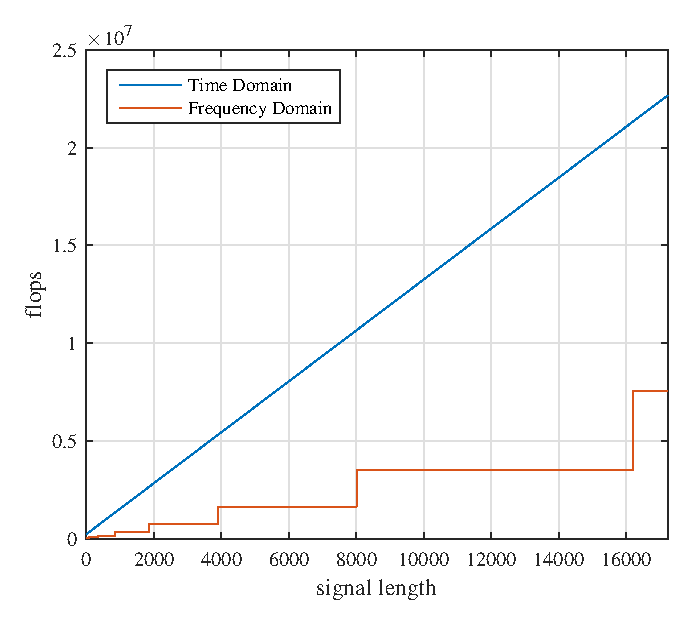
\includegraphics[width=5in]{figures/gpu_intro/Theory186Tap_flops.eps}
	\caption{Comparison of number of floating point operations (flops) required to convolve a variable length complex signal with a $186$ tap complex filter.}
	\label{fig:Theory186Tap_flops}
\end{figure}
\begin{figure}
	\centering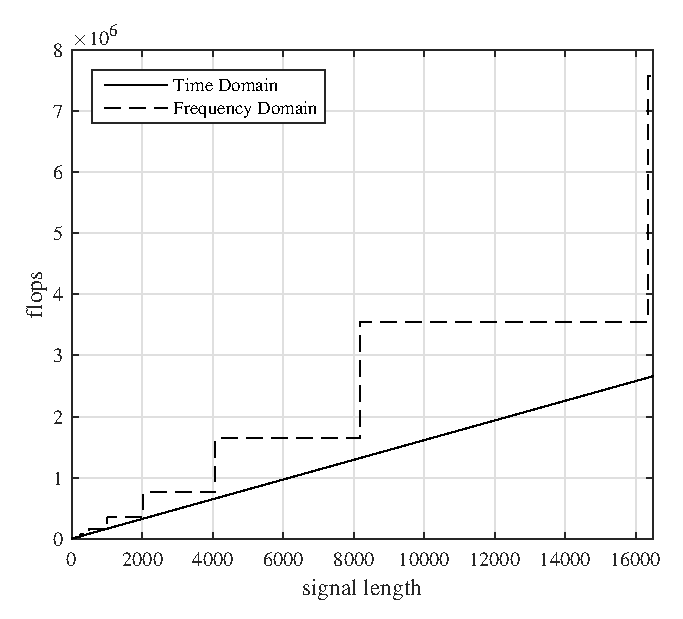
\includegraphics[width=5in]{figures/gpu_intro/Theory23Tap_flops.eps}
	\caption{Comparison of number of floating point operations (flops) required to convolve a variable length complex signal with a $23$ tap complex filter.}
	\label{fig:Theory23Tap_flops}
\end{figure}
\begin{figure} 
	\centering\includegraphics[width=5in]{figures/gpu_intro/Theory12672signal_flops.eps}
	\caption{Comparison of number of floating point operations (flops) required to convolve a $12$,$672$ sample complex signal with a variable length tap complex filter.}
	\label{fig:Theory12672signal_flops}
\end{figure}

\subsection{CPU and GPU Single Convolution Using Batch Processing Comparison}
\label{sec:cuda_convolution_single}
This section will show GPU convolution execution time is dependent more on memory access than the number of required floating point operations, while CPU convolution execution time is dependent on the number of floating point operations.
To illustrate these points, the execution time of the code in Listing \ref{code:convFun} (at the end of the chapter) was measured.
The code implements convolution five different ways:
\begin{itemize}
  \item time-domain convolution in a CPU,
  \item frequency-domain convolution in a CPU using the FFTW library,
  \item time-domain convolution in a GPU using global memory,
  \item time-domain convolution in a GPU using shared memory, and
  \item frequency-domain convolution in a GPU using the cuFFT library.
\end{itemize}

The three time-domain convolution implementations compute \eqref{eq:simple_conv_time} directly.
The two \newline frequency-domain convolution implementations compute \eqref{eq:simple_conv_freq}, using the CPU FFTW library and the GPU based cuFFT library.
The cuFFT library uses global memory and shared memory to be as fast and efficient as possible.
For a given signal and filter length, a good CUDA programmer can make an educated guess on which algorithm is faster.
There is no clear conclusion, until all the algorithms have been implemented and measured.

%The CPU implements Equation \eqref{eq:simple_conv_time} in ConvCPU directly on line $209$ using a function from lines $11$ to $34$.
%The CPU implements Equation \eqref{eq:simple_conv_freq} using the FFTW library on lines $214$ to $258$.
%
%The GPU implements time-domain convolution using global memory in lines $268$ to $277$.
%The GPU kernel ConvGPU on lines $36$ to $64$ is a parallel version of ConvCPU.
%ConvGPU performs time-domain convolution by fetching every element of the signal and filter from global memory.
%
%The GPU implements time-domain convolution using shared memory in lines $283$ to $292$.
%The GPU kernel ConvGPUshared on lines $67$ to $101$ is nearly identical to ConvGPU.
%Threads accessing the same elements of the filter in global memory can be a waste of valuable clock cycles.
%ConvGPUshared pays and initial price on lines $72$ to $76$ to move $L_\text{h}$ filter coefficients from off chip global memory to the on chip shared memory.
%Finally, the GPU implements frequency-domain convolution using the cuFFT library on lines $298$ to $326$.
%
%The questions are:
%Do flops have a direct relationship to execution time on CPUs? 
%Do flops have a direct relationship to execution time on GPUs? 
%When is the initial cost to use shared memory worth it?
%When should convolution be done in the frequency domain?
%
%The short answer to all of the questions is: GPU execution time depend on the signal length, filter length, CPU, GPU and memory.
%A good CUDA programmer can make an educated guess on which algorithm may be faster in the GPU, but until all the algorithms have been implemented and timed, there is no definite answer.

All the memory transfers to and from the GPU were timed for a fair comparison of GPU to CPU execution time.
Table \ref{tab:CPUvsGPUtimingTable} shows how the execution time was measured for each convolution implementation.
\begin{table}
\caption{Defining start and stop lines for timing comparison in Listing \ref{code:convFun}.}
\begin{center}
\begin{tabular}{llll}
	\toprule
	Algorithm 				& Function		& Start Line	& Stop  Line		\\ \midrule
	CPU time domain 		& ConvCPU 		& 208			& 210 				\\
	CPU frequency domain 	& FFTW 			& 213			& 259 				\\
	GPU time domain global 	& ConvGPU 		& 267			& 278				\\
	GPU time domain shared 	& ConvGPUshared & 282			& 293				\\
	GPU frequency domain 	& cuFFT			& 301			& 327				\\ 
	\bottomrule
\end{tabular}
\end{center}
\label{tab:CPUvsGPUtimingTable}
\end{table}
Figures \ref{fig:CPUvsGPU_1batch_186taps_varySignal_noMin} through \ref{fig:CPUvsGPU_1batch_12672signal_varyFilter} compare execution time of the five different convolution implementations by fixing the filter length with variable signal length or vise versa.
Sub-windows emphasize points that are of interest to the PAQ system.
The variations in the time-domain CPU execution times are due to the claims on the host CPU resources by the operating system.
To clean up the time samples, local minima were found in windows ranging from 3 to 15 samples.
The smallest windows possible were used to produce the results.
\begin{figure}
	\centering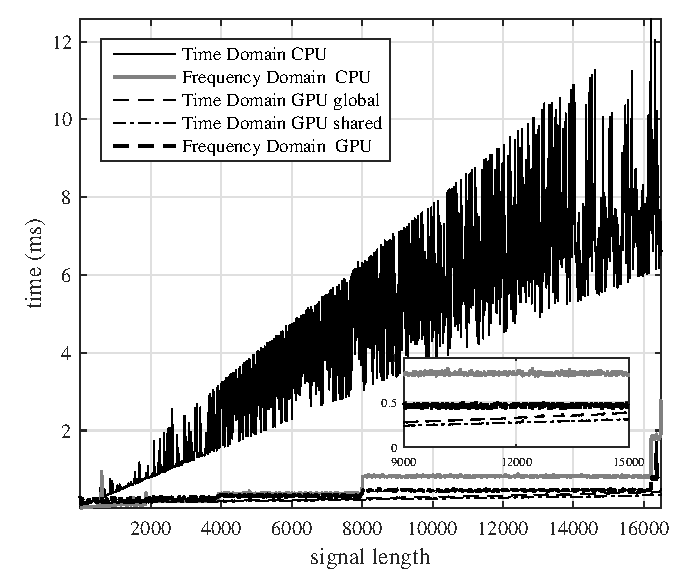
\includegraphics[width=5in]{figures/gpu_intro/CPUvsGPU_1batch_186taps_varySignal_noMin.eps}
	\caption{Comparison of a complex convolution on CPU and GPU. The signal length is variable and the filter is fixed at $186$ taps. The comparison is messy without lower bounding.}
	\label{fig:CPUvsGPU_1batch_186taps_varySignal_noMin}
\end{figure}
\begin{figure}
	\centering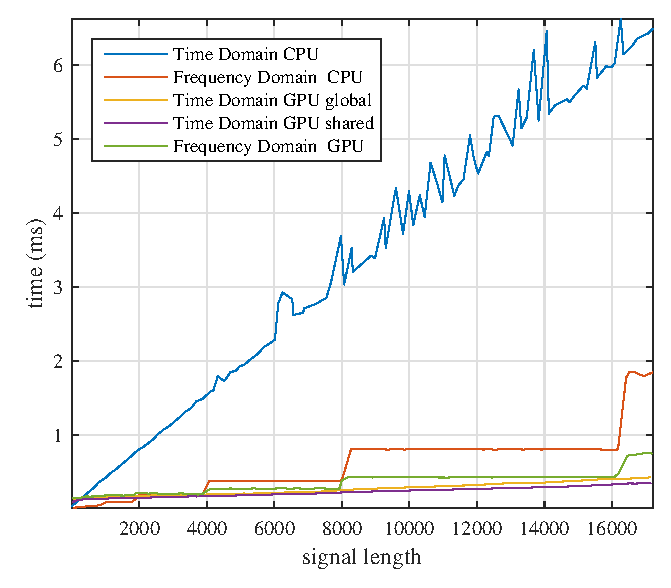
\includegraphics[width=5in]{figures/gpu_intro/CPUvsGPU_1batch_186taps_varySignal.eps}
	\caption{Comparison of a complex convolution on CPU and GPU. The signal length is variable and the filter is fixed at $186$ taps. A lower bound was applied by searching for a local minima in 15 sample width windows.}
	\label{fig:CPUvsGPU_1batch_186taps_varySignal}
\end{figure}
\begin{figure}
	\centering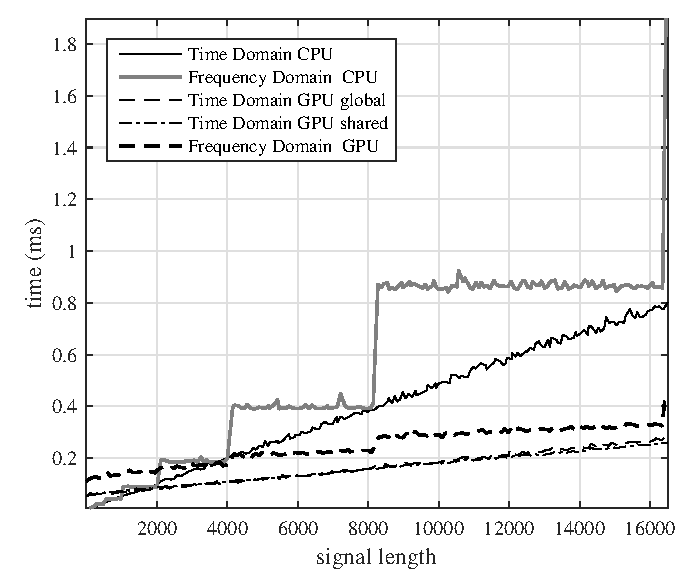
\includegraphics[width=5in]{figures/gpu_intro/CPUvsGPU_1batch_23taps_varySignal.eps}
	\caption{Comparison of a complex convolution on CPU and GPU. The signal length is variable and the filter is fixed at $23$ taps. A lower bound was applied by searching for a local minima in 5 sample width windows.}
	\label{fig:CPUvsGPU_1batch_23taps_varySignal}
\end{figure}
\begin{figure}
	\centering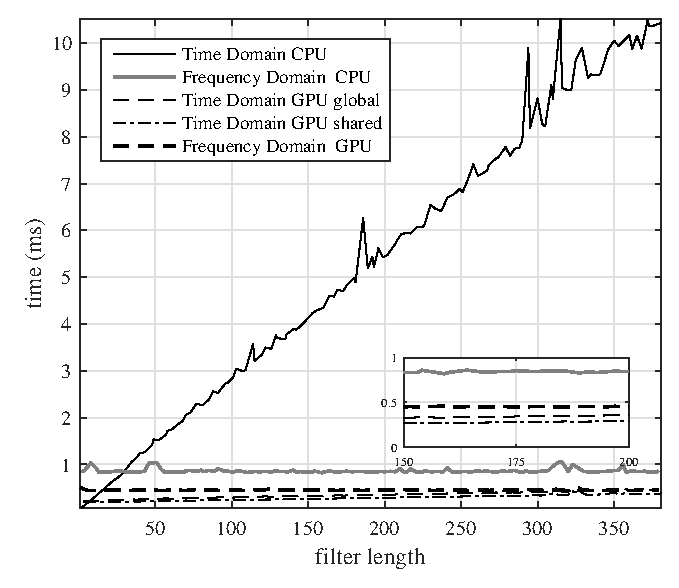
\includegraphics[width=5in]{figures/gpu_intro/CPUvsGPU_1batch_12672signal_varyFilter.eps}
	\caption{Comparison of a complex convolution on CPU and GPU. The filter length is variable and the signal is fixed at $12$,$672$ samples. A lower bound was applied by searching for a local minima in three sample width windows.}
	\label{fig:CPUvsGPU_1batch_12672signal_varyFilter}
\end{figure}

Comparing Figures \ref{fig:CPUvsGPU_1batch_186taps_varySignal} through \ref{fig:CPUvsGPU_1batch_12672signal_varyFilter}
to Figures \ref{fig:Theory186Tap_flops} through
\ref{fig:Theory12672signal_flops} 
shows
CPU and GPU convolution have the same structure that the number of flops predicted, except GPU convolution is not affected as much by varied signal or filter lengths.
The convolution execution time comparison demonstrates the observation that most GPU kernels execution time is limited by memory bandwidth not computational resources.
Tables \ref{tab:CPUvsGPUtable_12672_186} and \ref{tab:CPUvsGPUtable_12672_23} show the GPU time-domain algorithm using shared memory is fastest for the signal length and filter lengths of the PAQ system, when performing a single complex convolution.
\begin{table}
\caption{Convolution computation times with signal length $12$,$672$ and filter length $186$ on a Tesla K40c GPU.}
\begin{center}
\begin{tabular}{lll}
	\toprule
	Algorithm 				& Function or Library		& Execution Time (ms) \\ \midrule
	CPU time domain 		& ConvCPU 					& 6.2683		\\
	CPU frequency domain 	& FFTW 						& 0.8519		\\
	GPU time domain global 	& ConvGPU 					& 0.3467		\\
	GPU time domain shared 	& ConvGPUshared 			& 0.2857		\\
	GPU frequency domain 	& cuFFT						& 0.4490		\\ 
	\bottomrule
\end{tabular}
\end{center}
\label{tab:CPUvsGPUtable_12672_186}
\end{table}
\begin{table}
\caption{Convolution computation times with signal length $12$,$672$ and filter length $23$ on a Tesla K40c GPU.}
\begin{center}
\begin{tabular}{lll}
	\toprule
	Algorithm 				& Function or Library		& Execution Time (ms) \\ \midrule
%	CPU time domain 		& ConvCPU 					& 0.5878		\\
%	CPU frequency domain 	& FFTW 						& 0.8417		\\
%	GPU time domain global 	& ConvGPU 					& 0.4476		\\
%	GPU time domain shared 	& ConvGPUshared 			& 0.1971		\\
%	GPU frequency domain 	& cuFFT						& 0.3360		\\
	CPU time domain 		& ConvCPU 					& 0.6429		\\
	CPU frequency domain 	& FFTW 						& 0.8899		\\
	GPU time domain global 	& ConvGPU 					& 0.2406		\\
	GPU time domain shared 	& ConvGPUshared 			& 0.2346		\\
	GPU frequency domain 	& cuFFT						& 0.3231		\\
	\bottomrule
\end{tabular}
\end{center}
\label{tab:CPUvsGPUtable_12672_23}
\end{table}

\subsection{Convolution Using Batch Processing}
\label{sec:batched_convolution}
Section \ref{sec:cuda_convolution_single}, illustrated convolving one signal with one filter, does not leverage the full power of parallel processing in GPUs.
The received signal in the PAQ system has a packetized structure with $3104$ packets per $1907$ ms.
Rather than processing each packet separately, the packets may be buffered and processed in a batch.
Batch processing in GPUs has less CPU overhead and introduces an extra level of parallelism.
Batch processing has faster execution time per packet, than processing packets separately.
CUDA has many libraries that have batch processing, including cuFFT, cuBLAS and cuSolverSp.
Haidar et al. \cite{haidar2015optimization} showed batched libraries achieve more Gflops, than calling GPU kernels multiple times.
Listing \ref{code:batchedConvFun} (at the end of the chapter) shows three GPU implementations of convolution using batch processing and Table \ref{tab:BatchedGPUtimingTable} shows how the execution time of the code was measured.
\begin{table}
\caption{Defining start and stop lines for execution time comparison in Listing \ref{code:batchedConvFun}.}
\begin{center}
\begin{tabular}{llll}
	\toprule
	Algorithm 				& Function		& Start Line	& Stop  Line		\\ \midrule
	GPU time domain global 	& ConvGPU 		& 197			& 204				\\
	GPU time domain shared 	& ConvGPUshared & 212			& 219				\\
	GPU frequency domain 	& cuFFT			& 227			& 245				\\ 
	\bottomrule
\end{tabular}
\end{center}
\label{tab:BatchedGPUtimingTable}
\end{table}

Figure \ref{fig:CPUvsGPU_varyBatches_186taps_12672signal} compares execution time of convolution using batch processing as the number of packets increases, note that no lower bounding was used.
This figure shows that frequency-domain convolution leverages batch processing better than time-domain convolution.
As expected, CPU-based convolution using batch processing is not competitive with GPU-based convolution using batch processing and thus CPU-batched processing is not explored any further.
\begin{figure}
	\centering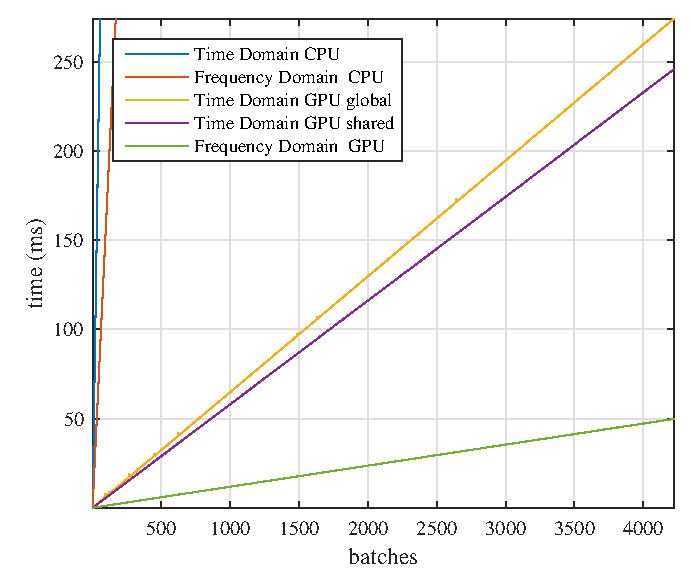
\includegraphics[width=5in]{figures/gpu_intro/CPUvsGPU_varyBatches_186taps_12672signal.eps}
	\caption{Comparison of a batched complex convolution on a CPU and GPU. The number of batches is variable while the signal and filter length is set to $12$,$672$ and $186$.}
	\label{fig:CPUvsGPU_varyBatches_186taps_12672signal}
\end{figure}

Now that the GPU and CPU execution time is not being compared, Table \ref{tab:BatchedGPUtimingTable} shows execution times include only GPU kernels and exclude memory transfers.
Figure \ref{fig:CPUvsGPU_varyBatches_186taps_12672signal_timePerBatch} compares GPU convolution using batch processing execution time per batch as the number of packets increases.
The figure shows execution time per batch decreases as the number of packets increases but stops improving after 70 packets.
\begin{figure}
	\centering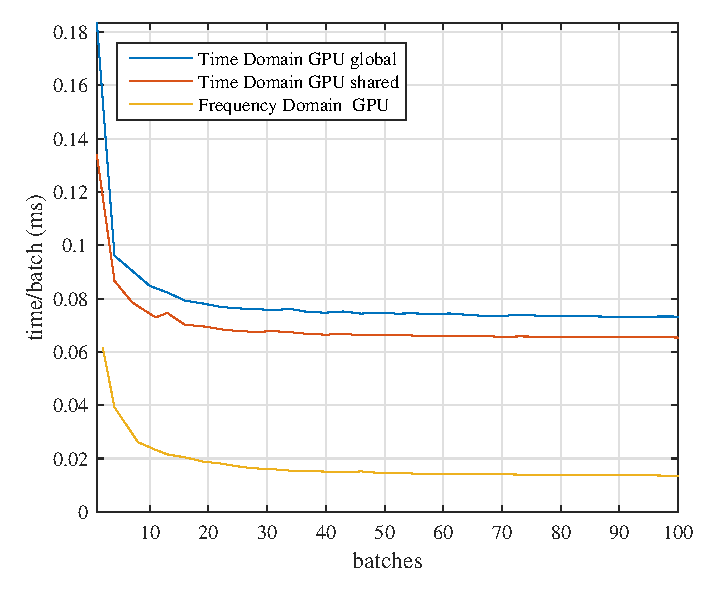
\includegraphics[width=5in]{figures/gpu_intro/CPUvsGPU_varyBatches_186taps_12672signal_timePerBatch.eps}
	\caption{Comparison on execution time per batch for complex convolution. The number of batches is variable while the signal and filter length is set to $12$,$672$ and $186$.}
	\label{fig:CPUvsGPU_varyBatches_186taps_12672signal_timePerBatch}
\end{figure}


Figures \ref{fig:CPUvsGPU_3104batch_186taps_varySignal} through \ref{fig:CPUvsGPU_3104batch_12672signal_varyFilter} 
compare execution time of the three GPU convolution implementations by fixing the filter length with variable signal length or vise versa.
Tables \ref{tab:Batched_CPUvsGPUtable_12672_186} and \ref{tab:Batched_CPUvsGPUtable_12672_23} 
show the execution times for the signal length and filter lengths of the PAQ system when performing convolution using batch processing.
Frequency-domain convolution using batch processing is fastest for $186$ tap filters while 
time-domain convolution using batch processing and shared memory is fastest for $23$ tap filters.
\begin{figure}
	\centering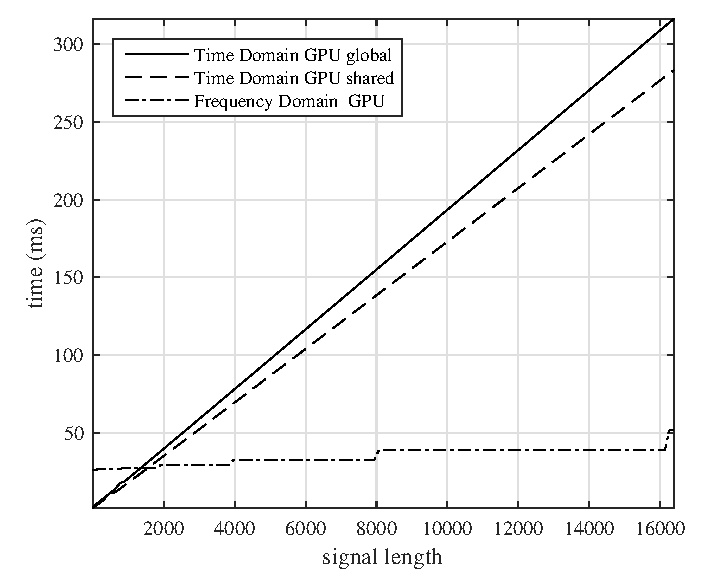
\includegraphics[width=5in]{figures/gpu_intro/CPUvsGPU_3104batch_186taps_varySignal.eps}
	\caption{Comparison of complex convolution using batch processing on a GPU. The signal length is variable and the filter is fixed at $186$ taps.}
	\label{fig:CPUvsGPU_3104batch_186taps_varySignal}
\end{figure}
\begin{figure}
	\centering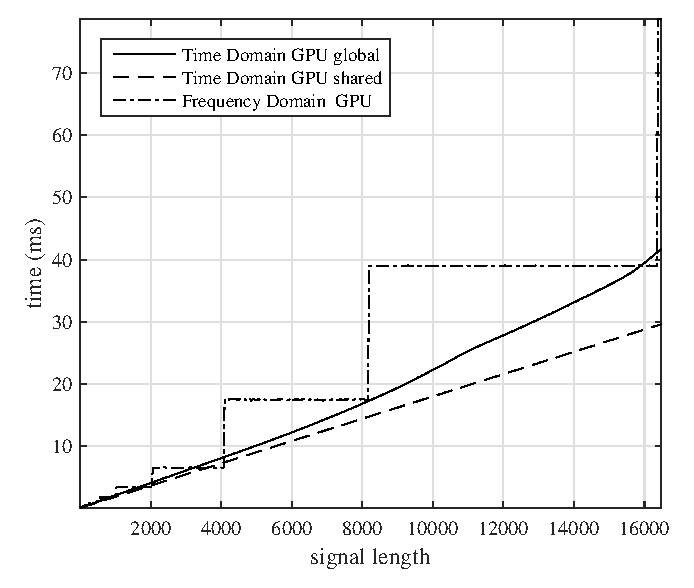
\includegraphics[width=5in]{figures/gpu_intro/CPUvsGPU_3104batch_23taps_varySignal.eps}
	\caption{Comparison of complex convolution using batch processing on a GPU. The signal length is variable and the filter is fixed at $23$ taps.}
	\label{fig:CPUvsGPU_3104batch_23taps_varySignal}
\end{figure}
\begin{figure}
	\centering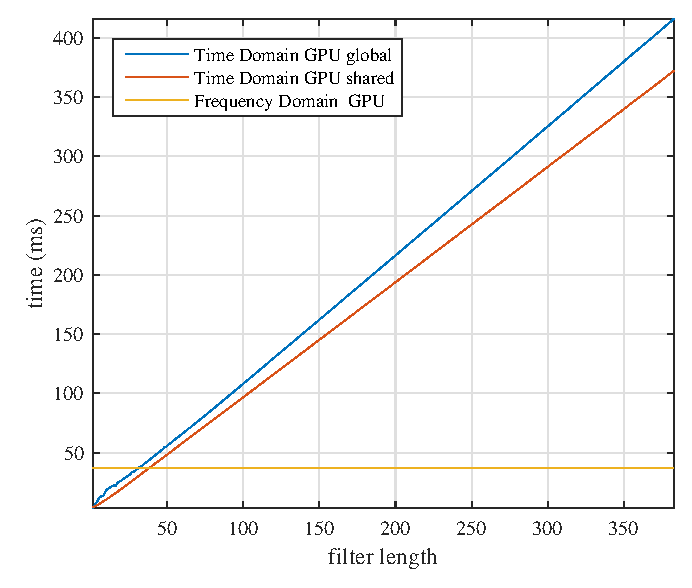
\includegraphics[width=5in]{figures/gpu_intro/CPUvsGPU_3104batch_12672signal_varyFilter.eps}
	\caption{Comparison of complex convolution using batch processing on a GPU. The filter length is variable and the signal length is set to $12$,$672$ samples.}
	\label{fig:CPUvsGPU_3104batch_12672signal_varyFilter}
\end{figure}
\begin{table}
\caption{Convolution using batch processing execution times with for a $12$,$672$ sample signal and $186$ tap filter on a Tesla K40c GPU.}
\begin{center}
\begin{tabular}{lll}
	\toprule
	Algorithm 				& Function or Library		& Execution Time (ms) \\ \midrule
	GPU time domain global 	& ConvGPU 					& 201.3		\\
	GPU time domain shared 	& ConvGPUshared 			& 180.3		\\
	GPU frequency domain 	& cuFFT						& 36.8 		\\ 
	\bottomrule
\end{tabular}
\end{center}
\label{tab:Batched_CPUvsGPUtable_12672_186}
\end{table}
\begin{table}
\caption{Convolution using batch processing execution times with for a $12$,$672$ sample signal and $23$ tap filter on a Tesla K40c GPU.}
\begin{center}
\begin{tabular}{lll}
	\toprule
	Algorithm 				& Function or Library		& Execution Time (ms) \\ \midrule
	GPU time domain global 	& ConvGPU 					& 29.5		\\
	GPU time domain shared 	& ConvGPUshared 			& 22.7			\\
	GPU frequency domain 	& cuFFT						& 39.0		\\ 
	\bottomrule
\end{tabular}
\end{center}
\label{tab:Batched_CPUvsGPUtable_12672_23}
\end{table}

Until now, convolving one signal with only one filter has been considered.
Figure \ref{fig:thisThesisBlock} showed the received signal is filtered by two cascaded filters: 
an equalizer filter and a detection filter.
The block diagrams in Figure \ref{fig:freq_time_block_cascade} show the steps required for cascading time-domain and frequency-domain convolution.

Comparing the block diagrams in Figures \ref{fig:freq_time_block_cascade} and \ref{fig:freq_time_block}, cascading two filters in the frequency domain only requires an extra FFT and point-by-point complex multiplication, while cascading filters in the time domain requires two time-domain convolutions.
The first time-domain convolution produces a composite filter from the convolution of the $186$ sample equalizer filter with the $23$ tap detection filter.
The second time-domain convolution applies the composite $208 = 186 + 23 - 1$ tap filter to a $12$,$672$ sample signal.
Table \ref{tab:Batched_CPUvsGPUtable_12672_23_186} shows the execution times for the signal length and filter lengths of the PAQ system, when performing cascaded convolution using batch processing.
Cascaded-convolution using batch processing in the frequency domain is fastest.
\begin{figure}
	\centering\includegraphics[width=10.28in/100*55]{figures/gpu_convolution/CascadeConvBlock.pdf}
	\caption{Block diagrams showing showing cascaded time-domain convolution and frequency-domain convolution.}
	\label{fig:freq_time_block_cascade}
\end{figure}
\begin{table}
\caption{Batched convolution execution times with for a $12$,$672$ sample signal and cascaded $23$ and $186$ tap filter on a Tesla K40c GPU.}
\begin{center}
\begin{tabular}{lll}
	\toprule
	Algorithm 				& Function or Library		& Execution Time (ms) \\ \midrule
	GPU time domain global 	& ConvGPU 					& 228.8		\\
	GPU time domain shared 	& ConvGPUshared 			& 205.0		\\
	GPU frequency domain 	& cuFFT						& 39.0		\\ 
	\bottomrule
\end{tabular}
\end{center}
\label{tab:Batched_CPUvsGPUtable_12672_23_186}
\end{table}



\singlespacing
\clearpage
\begin{lstlisting}[style=myCUDAstyle,language=C++,caption={CUDA code to performing complex convolution five different ways: time domain CPU, frequency domain CPU time domain GPU, time domain GPU using shared memory and frequency domain GPU.},label={code:convFun}]
#include <iostream>
#include <stdlib.h>
#include <math.h>
#include <cufft.h>
#include <fstream>
#include <string>
#include <fftw3.h>
using namespace std;


void ConvCPU(cufftComplex* y,cufftComplex* x,cufftComplex* h,int Lx,int Lh){
	for(int yIdx = 0; yIdx < Lx+Lh-1; yIdx++){
		cufftComplex temp;
		temp.x = 0;
		temp.y = 0;
		for(int hIdx = 0; hIdx < Lh; hIdx++){
			int xAccessIdx = yIdx-hIdx;
			if(xAccessIdx>=0 && xAccessIdx<Lx){
				// temp += x[xAccessIdx]*h[hIdx];
				float A = x[xAccessIdx].x;
				float B = x[xAccessIdx].y;
				float C = h[hIdx].x;
				float D = h[hIdx].y;
				cufftComplex result;
				result.x = A*C-B*D;
				result.y = A*D+B*C;
				temp.x += result.x;
				temp.y += result.y;
			}
		}
		y[yIdx] = temp;
	}

}

__global__ void ConvGPU(cufftComplex* y,cufftComplex* x,cufftComplex* h,int Lx,int Lh){
	int yIdx = blockIdx.x*blockDim.x + threadIdx.x;

	int lastThread = Lx+Lh-1;

	// don't access elements out of bounds
	if(yIdx >= lastThread)
		return;

	cufftComplex temp;
	temp.x = 0;
	temp.y = 0;
	for(int hIdx = 0; hIdx < Lh; hIdx++){
		int xAccessIdx = yIdx-hIdx;
		if(xAccessIdx>=0 && xAccessIdx<Lx){
			// temp += x[xAccessIdx]*h[hIdx];
			float A = x[xAccessIdx].x;
			float B = x[xAccessIdx].y;
			float C = h[hIdx].x;
			float D = h[hIdx].y;
			cufftComplex result;
			result.x = A*C-B*D;
			result.y = A*D+B*C;
			temp.x += result.x;
			temp.y += result.y;
		}
	}
	y[yIdx] = temp;
}


__global__ void ConvGPUshared(cufftComplex* y,cufftComplex* x,cufftComplex* h,int Lx,int Lh){
	int yIdx = blockIdx.x*blockDim.x + threadIdx.x;

	int lastThread = Lx+Lh-1;

	extern __shared__ cufftComplex h_shared[];
	if(threadIdx.x < Lh){
		h_shared[threadIdx.x] = h[threadIdx.x];
	}
	__syncthreads();

	// don't access elements out of bounds
	if(yIdx >= lastThread)
		return;

	cufftComplex temp;
	temp.x = 0;
	temp.y = 0;
	for(int hIdx = 0; hIdx < Lh; hIdx++){
		int xAccessIdx = yIdx-hIdx;
		if(xAccessIdx>=0 && xAccessIdx<Lx){
			// temp += x[xAccessIdx]*h[hIdx];
			float A = x[xAccessIdx].x;
			float B = x[xAccessIdx].y;
			float C = h_shared[hIdx].x;
			float D = h_shared[hIdx].y;
			cufftComplex result;
			result.x = A*C-B*D;
			result.y = A*D+B*C;
			temp.x += result.x;
			temp.y += result.y;
		}
	}
	y[yIdx] = temp;
}

__global__ void PointToPointMultiply(cufftComplex* v0, cufftComplex* v1, int lastThread){
	int i = blockIdx.x*blockDim.x + threadIdx.x;

	// don't access elements out of bounds
	if(i >= lastThread)
		return;
	float A = v0[i].x;
	float B = v0[i].y;
	float C = v1[i].x;
	float D = v1[i].y;

	// (A+jB)(C+jD) = (AC-BD) + j(AD+BC)
	cufftComplex result;
	result.x = A*C-B*D;
	result.y = A*D+B*C;

	v0[i] = result;
}

__global__ void ScalarMultiply(cufftComplex* vec0, float scalar, int lastThread){
	int i = blockIdx.x*blockDim.x + threadIdx.x;

	// Don't access elements out of bounds
	if(i >= lastThread)
		return;
	cufftComplex scalarMult;
	scalarMult.x = vec0[i].x*scalar;
	scalarMult.y = vec0[i].y*scalar;
	vec0[i] = scalarMult;
}

int main(){
	int N = 1000;
	int L = 186;
	int C = N + L - 1;
	int M = pow(2, ceil(log(C)/log(2)));

	cufftComplex *mySignal1;
	cufftComplex *mySignal2;
	cufftComplex *mySignal2_fft;

	cufftComplex *myFilter1;
	cufftComplex *myFilter2;
	cufftComplex *myFilter2_fft;

	cufftComplex *myConv1;
	cufftComplex *myConv2;
	cufftComplex *myConv2_timeReversed;
	cufftComplex *myConv3;
	cufftComplex *myConv4;
	cufftComplex *myConv5;

	mySignal1      		= (cufftComplex*)malloc(N*sizeof(cufftComplex));
	mySignal2      		= (cufftComplex*)malloc(M*sizeof(cufftComplex));
	mySignal2_fft  		= (cufftComplex*)malloc(M*sizeof(cufftComplex));

	myFilter1      		= (cufftComplex*)malloc(L*sizeof(cufftComplex));
	myFilter2      		= (cufftComplex*)malloc(M*sizeof(cufftComplex));
	myFilter2_fft  		= (cufftComplex*)malloc(M*sizeof(cufftComplex));

	myConv1        		= (cufftComplex*)malloc(C*sizeof(cufftComplex));
	myConv2        		= (cufftComplex*)malloc(M*sizeof(cufftComplex));
	myConv2_timeReversed= (cufftComplex*)malloc(M*sizeof(cufftComplex));
	myConv3        		= (cufftComplex*)malloc(C*sizeof(cufftComplex));
	myConv4        		= (cufftComplex*)malloc(C*sizeof(cufftComplex));
	myConv5        		= (cufftComplex*)malloc(M*sizeof(cufftComplex));

	srand(time(0));
	for(int i = 0; i < N; i++){
		mySignal1[i].x = rand()%100-50;
		mySignal1[i].y = rand()%100-50;
	}

	for(int i = 0; i < L; i++){
		myFilter1[i].x = rand()%100-50;
		myFilter1[i].y = rand()%100-50;
	}

	cufftComplex *dev_mySignal3;
	cufftComplex *dev_mySignal4;
	cufftComplex *dev_mySignal5;

	cufftComplex *dev_myFilter3;
	cufftComplex *dev_myFilter4;
	cufftComplex *dev_myFilter5;

	cufftComplex *dev_myConv3;
	cufftComplex *dev_myConv4;
	cufftComplex *dev_myConv5;

	cudaMalloc(&dev_mySignal3, N*sizeof(cufftComplex));
	cudaMalloc(&dev_mySignal4, N*sizeof(cufftComplex));
	cudaMalloc(&dev_mySignal5, M*sizeof(cufftComplex));

	cudaMalloc(&dev_myFilter3, L*sizeof(cufftComplex));
	cudaMalloc(&dev_myFilter4, L*sizeof(cufftComplex));
	cudaMalloc(&dev_myFilter5, M*sizeof(cufftComplex));

	cudaMalloc(&dev_myConv3,   C*sizeof(cufftComplex));
	cudaMalloc(&dev_myConv4,   C*sizeof(cufftComplex));
	cudaMalloc(&dev_myConv5,   M*sizeof(cufftComplex));


	/**
	 * Time-domain Convolution CPU
	 */
	ConvCPU(myConv1,mySignal1,myFilter1,N,L);

	/**
	 * Frequency Domain Convolution CPU
	 */
	fftwf_plan forwardPlanSignal = fftwf_plan_dft_1d(M, (fftwf_complex*)mySignal2,    (fftwf_complex*)mySignal2_fft, 	   FFTW_FORWARD, FFTW_MEASURE);
	fftwf_plan forwardPlanFilter = fftwf_plan_dft_1d(M, (fftwf_complex*)myFilter2, 	 (fftwf_complex*)myFilter2_fft, 	   FFTW_FORWARD, FFTW_MEASURE);
	fftwf_plan backwardPlanConv  = fftwf_plan_dft_1d(M, (fftwf_complex*)mySignal2_fft,(fftwf_complex*)myConv2_timeReversed, FFTW_FORWARD, FFTW_MEASURE);

	cufftComplex zero; zero.x = 0; zero.y = 0;
	for(int i = 0; i < M; i++){
		if(i<N)
			mySignal2[i] = mySignal1[i];
		else
			mySignal2[i] = zero;

		if(i<L)
			myFilter2[i] = myFilter1[i];
		else
			myFilter2[i] = zero;
	}

	fftwf_execute(forwardPlanSignal);
	fftwf_execute(forwardPlanFilter);

	for (int i = 0; i < M; i++){
		// mySignal2_fft = mySignal2_fft*myFilter2_fft;
		float A = mySignal2_fft[i].x;
		float B = mySignal2_fft[i].y;
		float C = myFilter2_fft[i].x;
		float D = myFilter2_fft[i].y;
		cufftComplex result;
		result.x = A*C-B*D;
		result.y = A*D+B*C;
		mySignal2_fft[i] = result;
	}

	fftwf_execute(backwardPlanConv);

	// myConv2 from fftwf must be time reversed and scaled
	// to match Matlab, myConv1, myConv3, myConv4 and myConv5
	cufftComplex result;
	for (int i = 0; i < M; i++){
		result.x = myConv2_timeReversed[M-i].x/M;
		result.y = myConv2_timeReversed[M-i].y/M;
		myConv2[i] = result;
	}
	result.x = myConv2_timeReversed[0].x/M;
	result.y = myConv2_timeReversed[0].y/M;
	myConv2[0] = result;

	fftwf_destroy_plan(forwardPlanSignal);
	fftwf_destroy_plan(forwardPlanFilter);
	fftwf_destroy_plan(backwardPlanConv);


	/**
	 * Time-domain Convolution GPU Using Global Memory
	 */
	cudaMemcpy(dev_mySignal3, mySignal1, sizeof(cufftComplex)*N, cudaMemcpyHostToDevice);
	cudaMemcpy(dev_myFilter3, myFilter1, sizeof(cufftComplex)*L, cudaMemcpyHostToDevice);

	int T_B = 512;
	int B = C/T_B;
	if(C % T_B > 0)
		B++;
	ConvGPU<<<B, T_B>>>(dev_myConv3, dev_mySignal3, dev_myFilter3, N, L);

	cudaMemcpy(myConv3, dev_myConv3, C*sizeof(cufftComplex), cudaMemcpyDeviceToHost);


	/**
	 * Time-domain Convolution GPU Using Shared Memory
	 */
	cudaMemcpy(dev_mySignal4, mySignal1, sizeof(cufftComplex)*N, cudaMemcpyHostToDevice);
	cudaMemcpy(dev_myFilter4, myFilter1, sizeof(cufftComplex)*L, cudaMemcpyHostToDevice);

	T_B = 512;
	B = C/T_B;
	if(C % T_B > 0)
		B++;
	ConvGPUshared<<<B, T_B,L*sizeof(cufftComplex)>>>(dev_myConv4, dev_mySignal4, dev_myFilter4, N, L);

	cudaMemcpy(myConv4, dev_myConv4, C*sizeof(cufftComplex), cudaMemcpyDeviceToHost);


	/**
	 * Frequency-domain Convolution GPU
	 */
	cufftHandle plan;
	int n[1] = {M};
	cufftPlanMany(&plan,1,n,NULL,1,1,NULL,1,1,CUFFT_C2C,1);

	cudaMemset(dev_mySignal5, 0, 	     M*sizeof(cufftComplex));
	cudaMemset(dev_myFilter5, 0, 	     M*sizeof(cufftComplex));

	cudaMemcpy(dev_mySignal5, mySignal2, M*sizeof(cufftComplex), cudaMemcpyHostToDevice);
	cudaMemcpy(dev_myFilter5, myFilter2, M*sizeof(cufftComplex), cudaMemcpyHostToDevice);

	cufftExecC2C(plan, dev_mySignal5, dev_mySignal5, CUFFT_FORWARD);
	cufftExecC2C(plan, dev_myFilter5, dev_myFilter5, CUFFT_FORWARD);

	T_B = 512;
	B = M/T_B;
	if(M % T_B > 0)
		B++;
	PointToPointMultiply<<<B, T_B>>>(dev_mySignal5, dev_myFilter5, M);

	cufftExecC2C(plan, dev_mySignal5, dev_mySignal5, CUFFT_INVERSE);

	T_B = 128;
	B = M/T_B;
	if(M % T_B > 0)
		B++;
	float scalar = 1.0/((float)M);
	ScalarMultiply<<<B, T_B>>>(dev_mySignal5, scalar, M);

	cudaMemcpy(myConv5, dev_mySignal5, M*sizeof(cufftComplex), cudaMemcpyDeviceToHost);

	cufftDestroy(plan);

	free(mySignal1);
	free(mySignal2);

	free(myFilter1);
	free(myFilter2);

	free(myConv1);
	free(myConv2);
	free(myConv2_timeReversed);
	free(myConv3);
	free(myConv4);
	free(myConv5);
	fftwf_cleanup();

	cudaFree(dev_mySignal3);
	cudaFree(dev_mySignal4);
	cudaFree(dev_mySignal5);

	cudaFree(dev_myFilter3);
	cudaFree(dev_myFilter4);
	cudaFree(dev_myFilter5);

	cudaFree(dev_myConv3);
	cudaFree(dev_myConv4);
	cudaFree(dev_myConv5);

	return 0;
}
\end{lstlisting}
\doublespacing

\singlespacing
\clearpage
\begin{lstlisting}[style=myCUDAstyle,language=C++,caption={CUDA code to perform batched complex convolution three different ways in a GPU: time domain using global memory, time domain using shared memory and frequency domain GPU.},label={code:batchedConvFun}]
#include <cufft.h>
#include <iostream>
using namespace std;

__global__ void ConvGPU(cufftComplex* y_out,cufftComplex* x_in,cufftComplex* h_in,int Lx,int Lh,int maxThreads){
	int threadNum = blockIdx.x*blockDim.x + threadIdx.x;
	int convLength = Lx+Lh-1;

	// Don't access elements out of bounds
	if(threadNum >= maxThreads)
		return;

	int batch = threadNum/convLength;
	int yIdx  = threadNum%convLength;
	cufftComplex* x = &x_in[Lx*batch];
	cufftComplex* h = &h_in[Lh*batch];
	cufftComplex* y = &y_out[convLength*batch];

	cufftComplex temp;
	temp.x = 0;
	temp.y = 0;
	for(int hIdx = 0; hIdx < Lh; hIdx++){
		int xAccessIdx = yIdx-hIdx;
		if(xAccessIdx>=0 && xAccessIdx<Lx){
			// temp += x[xAccessIdx]*h[hIdx];
			// (A+jB)(C+jD) = (AC-BD) + j(AD+BC)
			float A = x[xAccessIdx].x;
			float B = x[xAccessIdx].y;
			float C = h[hIdx].x;
			float D = h[hIdx].y;
			cufftComplex complexMult;
			complexMult.x = A*C-B*D;
			complexMult.y = A*D+B*C;

			temp.x += complexMult.x;
			temp.y += complexMult.y;
		}
	}
	y[yIdx] = temp;
}

__global__ void ConvGPUshared(cufftComplex* y_out,cufftComplex* x_in,cufftComplex* h_in,int Lx,int Lh,int maxThreads){

	int threadNum = blockIdx.x*blockDim.x + threadIdx.x;
	int convLength = Lx+Lh-1;
	// Don't access elements out of bounds
	if(threadNum >= maxThreads)
		return;

	int batch = threadNum/convLength;
	int yIdx  = threadNum%convLength;
	cufftComplex* x = &x_in[Lx*batch];
	cufftComplex* h = &h_in[Lh*batch];
	cufftComplex* y = &y_out[convLength*batch];

	extern __shared__ cufftComplex h_shared[];
	if(threadIdx.x < Lh)
		h_shared[threadIdx.x] = h[threadIdx.x];

	__syncthreads();

	cufftComplex temp;
	temp.x = 0;
	temp.y = 0;
	for(int hIdx = 0; hIdx < Lh; hIdx++){
		int xAccessIdx = yIdx-hIdx;
		if(xAccessIdx>=0 && xAccessIdx<Lx){
			// temp += x[xAccessIdx]*h[hIdx];
			// (A+jB)(C+jD) = (AC-BD) + j(AD+BC)
			float A = x[xAccessIdx].x;
			float B = x[xAccessIdx].y;
			float C = h_shared[hIdx].x;
			float D = h_shared[hIdx].y;
			cufftComplex complexMult;
			complexMult.x = A*C-B*D;
			complexMult.y = A*D+B*C;

			temp.x += complexMult.x;
			temp.y += complexMult.y;
		}
	}
	y[yIdx] = temp;
}

__global__ void PointToPointMultiply(cufftComplex* vec0, cufftComplex* vec1, int maxThreads){
	int i = blockIdx.x*blockDim.x + threadIdx.x;
	// Don't access elements out of bounds
	if(i >= maxThreads)
		return;
	// vec0[i] = vec0[i]*vec1[i];
	// (A+jB)(C+jD) = (AC-BD) + j(AD+BC)
	float A = vec0[i].x;
	float B = vec0[i].y;
	float C = vec1[i].x;
	float D = vec1[i].y;
	cufftComplex complexMult;
	complexMult.x = A*C-B*D;
	complexMult.y = A*D+B*C;
	vec0[i] = complexMult;
}

__global__ void ScalarMultiply(cufftComplex* vec0, float scalar, int lastThread){
	int i = blockIdx.x*blockDim.x + threadIdx.x;
	// Don't access elements out of bounds
	if(i >= lastThread)
		return;
	cufftComplex scalarMult;
	scalarMult.x = vec0[i].x*scalar;
	scalarMult.y = vec0[i].y*scalar;
	vec0[i] = scalarMult;
}

int main(){
	int numBatches = 3104;
	int N = 12672;
	int L = 186;
	int C = N + L - 1;
	int M = pow(2, ceil(log(C)/log(2)));
	int maxThreads;
	int T_B;
	int B;

	cufftHandle plan;
	int n[1] = {M};
	cufftPlanMany(&plan,1,n,NULL,1,1,NULL,1,1,CUFFT_C2C,numBatches);

	// Allocate memory on host
	cufftComplex *mySignal1;
	cufftComplex *mySignal1_pad;
	cufftComplex *myFilter1;
	cufftComplex *myFilter1_pad;
	cufftComplex *myConv1;
	cufftComplex *myConv2;
	cufftComplex *myConv3;
	mySignal1      = (cufftComplex*) malloc(N*numBatches*sizeof(cufftComplex));
	mySignal1_pad  = (cufftComplex*) malloc(M*numBatches*sizeof(cufftComplex));
	myFilter1      = (cufftComplex*) malloc(L*numBatches*sizeof(cufftComplex));
	myFilter1_pad  = (cufftComplex*) malloc(M*numBatches*sizeof(cufftComplex));
	myConv1        = (cufftComplex*) malloc(C*numBatches*sizeof(cufftComplex));
	myConv2        = (cufftComplex*) malloc(C*numBatches*sizeof(cufftComplex));
	myConv3        = (cufftComplex*) malloc(M*numBatches*sizeof(cufftComplex));

	srand(time(0));
	for(int i = 0; i < N; i++){
		mySignal1[i].x = rand()%100-50;
		mySignal1[i].y = rand()%100-50;
	}

	for(int i = 0; i < L; i++){
		myFilter1[i].x = rand()%100-50;
		myFilter1[i].y = rand()%100-50;
	}

	cufftComplex zero;
	zero.x = 0;
	zero.y = 0;
	for(int i = 0; i<M*numBatches; i++){
		mySignal1_pad[i] = zero;
		myFilter1_pad[i] = zero;
	}
	for(int batch=0; batch < numBatches; batch++){
		for(int i = 0; i < N; i++){
			mySignal1[batch*N+i] = mySignal1[i];
			mySignal1_pad[batch*M+i] = mySignal1[i];
		}
		for(int i = 0; i < L; i++){
			myFilter1[batch*L+i] = myFilter1[i];
			myFilter1_pad[batch*M+i] = myFilter1[i];
		}
	}

	// Allocate memory on device
	cufftComplex *dev_mySignal1;
	cufftComplex *dev_mySignal2;
	cufftComplex *dev_mySignal3;
	cufftComplex *dev_myFilter1;
	cufftComplex *dev_myFilter2;
	cufftComplex *dev_myFilter3;
	cufftComplex *dev_myConv1;
	cufftComplex *dev_myConv2;
	cufftComplex *dev_myConv3;
	cudaMalloc(&dev_mySignal1, N*numBatches*sizeof(cufftComplex));
	cudaMalloc(&dev_mySignal2, N*numBatches*sizeof(cufftComplex));
	cudaMalloc(&dev_mySignal3, M*numBatches*sizeof(cufftComplex));
	cudaMalloc(&dev_myFilter1, L*numBatches*sizeof(cufftComplex));
	cudaMalloc(&dev_myFilter2, L*numBatches*sizeof(cufftComplex));
	cudaMalloc(&dev_myFilter3, M*numBatches*sizeof(cufftComplex));
	cudaMalloc(&dev_myConv1,   C*numBatches*sizeof(cufftComplex));
	cudaMalloc(&dev_myConv2,   C*numBatches*sizeof(cufftComplex));
	cudaMalloc(&dev_myConv3,   M*numBatches*sizeof(cufftComplex));

	/**
	 * Time-domain Convolution GPU Using Global Memory
	 */
	cudaMemcpy(dev_mySignal1, mySignal1, numBatches*sizeof(cufftComplex)*N, cudaMemcpyHostToDevice);
	cudaMemcpy(dev_myFilter1, myFilter1, numBatches*sizeof(cufftComplex)*L, cudaMemcpyHostToDevice);

	maxThreads = C*numBatches;
	T_B = 128;
	B = maxThreads/T_B;
	if(maxThreads % T_B > 0)
		B++;
	ConvGPU<<<B, T_B>>>(dev_myConv1, dev_mySignal1, dev_myFilter1, N, L, maxThreads);

	cudaMemcpy(myConv1, dev_myConv1, C*numBatches*sizeof(cufftComplex), cudaMemcpyDeviceToHost);

	/**
	 * Time-domain Convolution GPU Using Shared Memory
	 */
	cudaMemcpy(dev_mySignal2, mySignal1, numBatches*sizeof(cufftComplex)*N, cudaMemcpyHostToDevice);
	cudaMemcpy(dev_myFilter2, myFilter1, numBatches*sizeof(cufftComplex)*L, cudaMemcpyHostToDevice);

	maxThreads = C*numBatches;
	T_B = 256;
	B = maxThreads/T_B;
	if(maxThreads % T_B > 0)
		B++;
	ConvGPUshared<<<B, T_B, L*sizeof(cufftComplex)>>>(dev_myConv2, dev_mySignal2, dev_myFilter2, N, L,maxThreads);

	cudaMemcpy(myConv2, dev_myConv2, C*numBatches*sizeof(cufftComplex), cudaMemcpyDeviceToHost);

	/**
	 * Frequency-domain Convolution GPU
	 */
	cudaMemcpy(dev_mySignal3, mySignal1_pad, M*numBatches*sizeof(cufftComplex), cudaMemcpyHostToDevice);
	cudaMemcpy(dev_myFilter3, myFilter1_pad, M*numBatches*sizeof(cufftComplex), cudaMemcpyHostToDevice);

	cufftExecC2C(plan, dev_mySignal3, dev_mySignal3, CUFFT_FORWARD);
	cufftExecC2C(plan, dev_myFilter3, dev_myFilter3, CUFFT_FORWARD);

	maxThreads = M*numBatches;
	T_B = 96;
	B = maxThreads/T_B;
	if(maxThreads % T_B > 0)
		B++;
	PointToPointMultiply<<<B, T_B>>>(dev_mySignal3, dev_myFilter3, maxThreads);
	cufftExecC2C(plan, dev_mySignal3, dev_mySignal3, CUFFT_INVERSE);

	T_B = 640;
	B = maxThreads/T_B;
	if(maxThreads % T_B > 0)
		B++;
	float scalar = 1.0/((float)M);
	ScalarMultiply<<<B, T_B>>>(dev_mySignal3, scalar, maxThreads);

	cudaMemcpy(myConv3, dev_mySignal3, M*numBatches*sizeof(cufftComplex), cudaMemcpyDeviceToHost);

	cufftDestroy(plan);

	// Free vectors on CPU
	free(mySignal1);
	free(myFilter1);
	free(myConv1);
	free(myConv2);
	free(myConv3);

	// Free vectors on GPU
	cudaFree(dev_mySignal1);
	cudaFree(dev_mySignal2);
	cudaFree(dev_mySignal3);
	cudaFree(dev_myFilter1);
	cudaFree(dev_myFilter2);
	cudaFree(dev_myFilter3);
	cudaFree(dev_myConv1);
	cudaFree(dev_myConv2);
	cudaFree(dev_myConv3);

	return 0;
}
\end{lstlisting}
\doublespacing